% =====================================================================
%  УХААЛАГ COFFEESHOP-ЫН NFC СУУРИЛСАН ЗАХИАЛГЫН СИСТЕМ
%  Төслийн тайлан
%
%  Компайл: xelatex main.tex (2 удаа) — MiKTeX эсвэл TeX Live дээр =====================================================================
\documentclass[12pt,a4paper]{report}

% ---------------------- Фонт (кирилл дэмжлэгтэй) ----------------------
\usepackage{fontspec}
\setmainfont{Times New Roman}
\setsansfont{Arial}
\setmonofont{Consolas}[Scale=0.92]

% ---------------------- Хуудасны тохиргоо ----------------------
\usepackage[a4paper,top=20mm,bottom=20mm,left=30mm,right=15mm]{geometry}
\usepackage{setspace}
\onehalfspacing
\setlength{\parindent}{1.25cm}
\setlength{\parskip}{2pt}

% ---------------------- Багцууд ----------------------
\usepackage{graphicx}
\usepackage{babel}
\babelprovide[main, import]{mongolian}
\tolerance=2000
\emergencystretch=2em
\usepackage{xcolor}
\usepackage{booktabs}
\usepackage{amsmath}
\usepackage{array}
\usepackage{enumitem}
\usepackage{caption}
\usepackage{titlesec}
\usepackage{fancyhdr}
\usepackage{tikz}
\usetikzlibrary{arrows.meta,positioning,shapes.geometric,calc,fit,backgrounds}
\usepackage[hidelinks]{hyperref}

% ---------------------- Монгол гарчгууд ----------------------
\renewcommand{\contentsname}{АГУУЛГА}
\renewcommand{\listfigurename}{ЗУРГИЙН ЖАГСААЛТ}
\renewcommand{\listtablename}{ХҮСНЭГТИЙН ЖАГСААЛТ}
\renewcommand{\figurename}{Зураг}
\renewcommand{\tablename}{Хүснэгт}
\renewcommand{\chaptername}{Бүлэг}
\renewcommand{\bibname}{НОМ ЗҮЙ}

% ---------------------- Гарчгийн хэв маяг ----------------------
\titleformat{\chapter}[display]
  {\centering\normalfont\bfseries}
  {\chaptertitlename~\thechapter}{14pt}{\Large\MakeUppercase}
\titlespacing*{\chapter}{0pt}{-10pt}{24pt}
\titleformat{\section}{\normalfont\large\bfseries}{\thesection.}{0.6em}{}
\titleformat{\subsection}{\normalfont\normalsize\bfseries}{\thesubsection.}{0.5em}{}
\titlespacing*{\section}{0pt}{14pt}{8pt}
\titlespacing*{\subsection}{0pt}{10pt}{6pt}

% ---------------------- Хуудасны дугаар (доод төвд) ----------------------
\pagestyle{fancy}
\fancyhf{}
\renewcommand{\headrulewidth}{0pt}
\fancyfoot[C]{\thepage}
\fancypagestyle{plain}{%
  \fancyhf{}\renewcommand{\headrulewidth}{0pt}\fancyfoot[C]{\thepage}}

% ---------------------- Caption ----------------------
\captionsetup{font=small, labelfont=bf}
\captionsetup[table]{position=above}

% ---------------------- TikZ хэв маяг ----------------------
\tikzset{
  uc/.style={draw, ellipse, align=center, minimum width=2.4cm,
             minimum height=0.8cm, font=\small, fill=white},
  layer/.style={draw, rounded corners=3mm, fill=gray!8, inner sep=9pt},
  layerlbl/.style={font=\small\bfseries, anchor=north west},
  svc/.style={draw, rounded corners=1.5mm, fill=white,
              minimum height=0.85cm, align=center, font=\small},
  ext/.style={svc, fill=orange!15, dashed},
  dbx/.style={svc, fill=blue!8},
  ent/.style={draw, align=left, font=\small, fill=blue!4, inner sep=5pt},
  msg/.style={-{Stealth[length=2.6mm]}, font=\scriptsize},
  ret/.style={-{Stealth[length=2.6mm]}, dashed, font=\scriptsize},
  note/.style={draw, fill=yellow!20, font=\scriptsize, align=left, inner sep=3pt},
  flowbox/.style={draw, rounded corners=1.5mm, fill=blue!8,
                  minimum height=0.95cm, align=center, font=\small},
  st/.style={draw, rounded corners=1mm, fill=green!10,
             minimum height=0.7cm, font=\small\strut},
}

% Хэрэглэгчийн тохиолдлын диаграмм дахь актор (хүн) зурах
\newcommand{\actor}[4]{%
  \begin{scope}[shift={(#2,#3)}]
    \draw[thick] (0,0.18) circle (0.17);
    \draw[thick] (0,0.01) -- (0,-0.52);
    \draw[thick] (-0.26,-0.16) -- (0.26,-0.16);
    \draw[thick] (0,-0.52) -- (-0.2,-0.84);
    \draw[thick] (0,-0.52) -- (0.2,-0.84);
    \node[font=\small\bfseries, anchor=north, align=center] at (0,-0.9) {#4};
    \coordinate (#1) at (0,-0.24);
  \end{scope}%
}

\hypersetup{
  pdftitle={Ухаалаг кофе шопын NFC-д суурилсан захиалгын систем — Төслийн төлөвлөгөө},
  pdfauthor={М.Мөнхдорж, Ү.Тамир, Б.Эрдэнэбаяр},
}

\begin{document}

% =====================================================================
%  НҮҮР ХУУДАС
% =====================================================================
\begin{titlepage}
  \centering
  {\large\bfseries ШИНЭ МОНГОЛ ТЕХНОЛОГИЙН ИХ СУРГУУЛЬ (ШМТИС)}\\[2.2cm]

  % Энд сургуулийн логоо хийнэ үү:
  % \includegraphics[width=3.2cm]{figures/logo.png}\\[2.2cm]

  {\Large\bfseries «УХААЛАГ КОФЕ ШОПЫН NFC-Д СУУРИЛСАН\\[6pt] ЗАХИАЛГЫН СИСТЕМ»}\\[12pt]
  {\normalsize --- Төслийн төлөвлөгөө ---}\\[2.2cm]

  \begin{tabular}{@{}p{3.2cm}@{}p{8.4cm}@{}}
    \textbf{Гүйцэтгэсэн:} & М.Мөнхдорж, Ү.Тамир, Б.Эрдэнэбаяр \\[10pt]
    \textbf{Удирдсан:}    &  ................................ \\

  \end{tabular}

  \vfill
  {\normalsize Улаанбаатар хот}\\[2pt]
  {\normalsize 2026 он}
\end{titlepage}

% =====================================================================
%  УГТГАЛ ХЭСЭГ (роман тоолол)
% =====================================================================
\pagenumbering{roman}

% =====================================================================
%  ХУРААНГУЙ (монгол) ба ABSTRACT (англи)
% =====================================================================
\chapter*{ХУРААНГУЙ}
\addcontentsline{toc}{chapter}{Хураангуй}

Энэхүү төслийн ажилд кофе шопын үйлчилгээний урсгалыг автоматжуулсан
ухаалаг захиалгын системийг NFC стикертэй хамт нэг цогц бүтээгдэхүүн
болгон боловсруулж, ажиллагаатай кофе шопуудад шууд борлуулах
бизнесийн төслийн баримт бичгийг бүрэн хэмжээгээр гаргав. Систем нь
зочин ширээн дээр байрлах NFC стикерийг гар утсаар уншуулснаар цахим
цэс автоматаар нээгдэж, захиалгаа өгч, төлбөрийг нэг цогц орчинд
төлснөөр захиалгаа ширээндээ хүргүүлж авах боломжийг олгоно.

Төслийн бизнесийн загвар нь үйлчилгээ үзүүлэх бус, бүтээгдэхүүнийг шууд
борлуулах зарчимд суурилна: кофе шоп бүрд ширээ тус бүрт нэг удаа NFC
стикер байршуулж, тухайн кофе шопын цэс болон холбогдох системийг
тохируулан өгснөөр ханган нийлүүлэлтийн ажил дуусна. Дараа нь кофе
шоп өөрийн админ эрхээр нэвтрэн цэсээ шинэчлэх -- шинэ бүтээгдэхүүн
нэмэх, хасах, үнийн өөрчлөлт оруулах боломжтой. Ингэж олон кофе шоптой
давтан ажиллаж, нэгж борлуулалт бүрээс ашиг олно.

Судалгааны хүрээнд кафе-ийн уламжлалт үйлчилгээний урсгалын бэрхшээлүүдийг
тодорхойлж, NFC, QR код, өөрөө үйлчлэх терминал (kiosk), аппликешнд
суурилсан шийдлүүдийг харьцуулан шинжилэв. Харьцуулалтаас үзвэл NFC стикер
нь ширээг автоматаар таних, нэг алхамаар цэс нээх, гадна орчны нөлөөнд
тэсвэртэй байх зэрэг давуу талыг өгөх бөгөөд орчин үеийн Android болон
iPhone утаснууд стикерийг арын дэвсгэртэд (background) унших чадвартай
тул тусгай аппликешн таталгүйгээр ашиглах боломжтойг харуулав.

Төслийн баримт бичигт төслийн танилцуулга, нөхцөл байдлын шинжилгээ,
маркетингийн төлөвлөгөө (нэг удаагийн багц үнийн бүтэцтэй), удирдлага,
зохион байгуулалт болон хүний нөөцийн төлөвлөгөө, системийн загвар,
санхүүгийн төлөвлөгөө, эрсдэлийн үнэлгээг багтаав. Системийн загварын
хүрээнд гурван давхаргат (клиент -- аппликешн -- өгөгдөл) архитектур,
NFC уншилтаас төлбөр баталгаажуулалт хүртэлх урсгалын диаграмм,
өгөгдлийн сангийн объект-харилцааны (ER) загвар, REST API-ийн
тодорхойлолт, аюулгүй байдлын загвар, туршилтын төлөвлөгөөг
багтаав. Хөгжүүлэлтийн технологиор React (PWA), NestJS, PostgreSQL,
Redis болон Docker-ийг сонгосон. Санхүүгийн урьдчилсан тооцоогоор
нийт хөрөнгө оруулалт 55.5 сая төгрөг буюу 3 жилийн дотор 171\%-ийн
хөрөнгө оруулалтын өгөөжтэй (ROI), ойролцоогоор 35 сарын дотор
бүрэн нөхөгдөхөөр байна.

\noindent\textbf{Түлхүүр үгс:} NFC, ухаалаг захиалгын систем, PWA,
REST API, төлбөрийн интеграци, бүтээгдэхүүний борлуулалт.

\chapter*{ABSTRACT}
\addcontentsline{toc}{chapter}{Abstract}

This project report presents the full business documentation for a
smart ordering system for coffee shops, developed together with an
NFC sticker as a single product and sold directly to operating coffee
shops. The system allows a customer to tap their phone on an NFC
sticker attached to the table, which opens a web-based menu with the
table automatically identified, place an order, and pay online so
that the order is delivered directly to their table --- without
standing in line at the counter.

The business model of the project is product-based direct sales
rather than a service: for each coffee shop, one NFC sticker is
installed on every table and the menu and related system are
configured for that shop, completing the delivery. Afterwards, the
coffee shop signs in with its own administrator account to update
its menu --- adding or removing products and changing prices. The
project earns profit by repeating this delivery across many coffee
shops.

The report analyses the shortcomings of the traditional counter-service
workflow and compares NFC-based identification with QR codes,
self-service kiosks and dedicated mobile applications. The analysis shows
that NFC stickers provide one-tap access to the menu, reliable table
identification, and high resilience to environmental conditions, while
modern Android and iPhone devices support background tag reading without
installing a dedicated application.

The document contains the project introduction, situation analysis,
marketing plan with a one-time package pricing structure, management
and human resources plan, system design, financial plan, and risk
assessment. The system design covers a three-tier architecture
(client --- application --- data), a diagram of the NFC-based order
and payment flow, an entity-relationship model of the database, a REST
API specification, a security design, and a test plan. React (PWA),
NestJS, PostgreSQL, Redis and Docker were selected as the
implementation technology stack. According to the preliminary financial
estimates, the total investment is 55.5 million MNT, with a three-year
return on investment (ROI) of 171\% and a full payback period of
approximately 35 months.

\noindent\textbf{Keywords:} NFC, smart ordering system, PWA, REST API,
payment integration, product sales.


\tableofcontents
\clearpage

% =====================================================================
%  ҮНДСЭН ХЭСЭГ (араб тоолол, 1-ээс)
% =====================================================================
\clearpage
\pagenumbering{arabic}
\setcounter{page}{1}

% =====================================================================
%  НЭГ. ТӨСЛИЙН ТАНИЛЦУУЛГА
% =====================================================================
\chapter{ТӨСЛИЙН ТАНИЛЦУУЛГА}

\section{Төслийн суурь үзүүлэлтүүд}

Төслийн суурь үзүүлэлтүүдийг Хүснэгт~\ref{tab:ch1-suur}~—т үзүүлэв.

\begin{table}[h]
  \centering
  \caption{Төслийн суурь үзүүлэлтүүд}
  \label{tab:ch1-suur}
  \begin{tabular}{@{}p{6.2cm}p{7.4cm}@{}}
    \toprule
    \textbf{Үзүүлэлт} & \textbf{Утга} \\ \midrule
    Төслийн нэр & «Ухаалаг кофе шопын NFC-д суурилсан захиалгын систем» \\
    Төсөл хэрэгжүүлэгч & М.Мөнхдорж, Ү.Тамир, Б.Эрдэнэбаяр \\
    Төслийн төрөл & Програм хангамжийн төсөл (бүтээгдэхүүний шууд
                      борлуулалттай) \\
    Хэрэгжих хугацаа & 6 сар (2026.10 -- 2027.03) \\
    Хөрөнгө оруулалтын хэмжээ & 55{,}533{,}896 төгрөг \\
    Төлөвлөж буй хүчин чадал & Нэг жилийн дотор 10 -- 20 кофе шопт
                               бүтээгдэхүүнээ борлуулах \\
    Цаашдын зорилго & Хот хөдөөгийн ялгаагүйгээр, улмаар гадаад зах зээлд
                      экспортлох \\
    \bottomrule
  \end{tabular}
\end{table}

\section{Төсөл хэрэгжүүлэгчийн тухай}

Төслийг Шинэ Монгол Технологийн Их Сургуулийн (ШМТИС) оюутнууд
М.Мөнхдорж, Ү.Тамир, Б.Эрдэнэбаяраас бүрдсэн баг бүтээн байгуулна. Баг
нь веб болон гар утасны аппликешн хөгжүүлэлт, өгөгдлийн сан, төслийн
удирдлагын чиглэлээр бэлтгэгдсэн гурван гишүүдээс бүрдэнэ. Багийн
гишүүд урьд өмнө веб болон гар утасны аппликешн хөгжүүлэх төслүүдэд
ажиллаж байсан туршлагатай, React, NestJS, PostgreSQL технологуудын
судалгааг тусгайлан хийсэн (\cite{react, nestjs, postgres}).

Санхүүгийн чадавх: Төслийн нийт хөрөнгө оруулалтын 50\% нь багийн
өөрийн санхүүгийн хөрөнгөөр, үлдсэн 50\% нь зээлийн хөрөнгөөр
хангагдана. Төслийн санхүүгийн урьдчилсан тооцоо нь хөрөнгө
оруулалтыг 35 сарын дотор нөхөхөд чиглэсэн бөгөөд нийлээд
санхүүгийн чадавх нь төслийг бүрэн хэрэгжүүлэхэд хүрэлцэхүйц болно.

\section{Төслийн тухай}

\subsection{Төслийн бүтээгдэхүүний танилцуулга}

Төслийн бүтээгдэхүүн нь кофе шопын ширээнд суусан хэрэглэгчид зориулсан
NFC стикер, PWA (Progressive Web App) маягийн цахим цэс, цахим
захиалга болон төлбөрийн системээс бүрдсэн цогц шийдэл юм. Хэрэглэгч
ширеэнд байрлах NFC стикерийг утсаар уншуулснаар тухайн ширээг
автоматаар тодорхойлж, цахим цэс нээгдэж, захиалгаа өгч, төлбөрийг
нутгаасаа төлснөөр захиалгаа ширээндээ хүргэж авна.

Төсөл хэрэгжүүлэгч баг үйлчилгээ үзүүлэгч бус, бүтээгдэхүүнийг шууд
борлуулах загвараар ажиллана. Ажилладаг кофе шоп бүрд нэг удаа
NFC стикерийг ширээ тус бүрт байршуулж, цэс болон холбогдох
системийг тухайн кофе шопт тохируулан өгснөөр манай ажил дуусна.
Дараа нь кофе шоп өөрийн админ эрхээр нэвтрэн цэсээ шинэчлэх --
шинэ бүтээгдэхүүн нэмэх, хасах, үнийн өөрчлөлт оруулах боломжтой.
Энэхүү загварыг олон кофе шоптой давтан хэрэгжүүлж, ашиг олно.

Бүтээгдэхүүний гол бүрэлдэхүүн хэсгүүд:

\begin{itemize}
  \item \textbf{NFC стикер (NTAG213/215):} Ширээ бүр дээр байрлах, тухайн
        ширээний дугаарыг кодчилсон стикер \cite{nxpntag}.
  \item \textbf{Хэрэглэгчийн PWA аппликешн:} Утасны арын дэвсгэртэд NFC
        уншиж, цэсийг нээх, захиалга өгөх, төлбөр төлөх интерфэйс \cite{androidnfc, corenfc}.
  \item \textbf{Кофе шопын админ хэсэг:} Цэс, үнийн сан, тайлан тооцоо,
        нэгжийн тохиргоог өөрөө удирдах бүрэн эрхт хэсэг.
  \item \textbf{Ажилтны хэсэг:} Захиалга хүлээн авах, гүйцэтгэх
        ажлын урсгалыг удирдах dashboard.
\end{itemize}

\subsection{Төслийн танилцуулга}

Уламжлалт кофе шопын үйлчилгээний урсгалд дараах бэрхшээлүүд
тархаж байна:

\begin{itemize}
  \item Кассын дээр хүн бөөгнөрч, үйлчлүүлэгчид удаан хүлээх.
  \item Төлбөрийн хэлбэр нь нэг удаагийн бөгөөд бичил болон бэлэн
        мөнгөний алдаа гарах боломжтой.
  \item Цэсээ хэвлэмэл хэлбэрээр харуулах нь өдөр тутмын хуучирал,
        засах зардлыг нэмэгдүүлдэг.
  \item Үйлчлүүлэгчийн мэдээллийг цуглуулж, үйлчилгээг хувь хүний
        тохирох боломжгүй.
\end{itemize}

Манай төсөл дээрх бэрхшээлүүдийг NFC технологи болон цахим төлбөрийн
системийг хослуулан шийдвэрлэнэ. Хэрэглэгчийн хөдөлгөөн дуусах хүртэлх
процессыг хурдасгаж, кофе шопын ажиллах хүчний ажлын ачааллыг бууруулж,
цаашид үйлчилгээний чанарыг нэмэгдүүлнэ.

\section{Төслийн үндсэн зорилго, зорилтууд}

\subsection{Төслийн зорилго, зорилтууд}

\textbf{Ерөнхий зорилго:} Кофе шопын үйлчилгээний урсгалыг NFC
технологиор автоматжуулан, хэрэглэгчид кассын дараалалгүйгээр захиалга
өгөх, төлөх, үйлчилгээг хүлээн авах нэгдсэн орчин бүрдүүлэх.

\textbf{Зорилтууд:}

\begin{enumerate}
  \item NFC стикерээр ширээг таних, цэсийг нэг алхамд нээх хэрэглэгчийн
        системийг бүрэн хэрэгжүүлэх.
  \item Захиалга өгөх, төлбөр төлөх, захиалгын төлөвийг хянах урсгалыг
        тасалдалгүйгээр холбох.
  \item Салбарын ажилтанд захиалгыг бодит цагт хүргэдэг хяналтын
        системийг боловсруулах.
  \item Бүрэн аюулгүй, хувийн мэдээллийг хамгаалсан архитектуртай
        системийг нэвтрүүлэх.
  \item Нэг жилийн дотор 10 -- 20 кофе шопт бүтээгдэхүүнээ
        борлуулж, системийн тогтвортой ажиллагааг батлах.
\end{enumerate}

\subsection{Төслийн ач холбогдол}

\begin{itemize}
  \item \textbf{Үйлчлүүлэгчид:} Хүлээх хугацааг 40 -- 50\% бууруулж,
        кассын дараалалгүй, нэг аппаар захиалга болон төлбөрийг
        гүйцэтгэх боломж.
  \item \textbf{Байгууллагад:} Кассын алдаа буурч, хүний нөөцийн
        ачаалал 20 -- 30\% хэмнэгдэнэ. Үйлчлүүлэгчийн мэдээлэл
        цуглуулагдаж, маркетингийн шийдвэр гаргалт илүү үр дүнтэй
        болно.
  \item \textbf{Салбарт:} Дотоодын компьютерийн технологийн
        бүтээгдэхүүний хомсдолыг нөхөж, уламжлалт бизнесийн салбарт
        цифржилтийг түлхүүлэх нөлөөтэй.
  \item \textbf{Эдийн засагт:} Уламжлалт үйлчилгээний салбарын
        урт хугацааны хэрэгцээнд чиглэсэн ажлын байр, технологийн
        шийдлийг дотоодын хүчээр бүтээх чадварыг нэмэгдүүлнэ.
\end{itemize}

% =====================================================================
%  ХОЁР. НӨХЦӨЛ БАЙДЛЫН ШИНЖИЛГЭЭ
% =====================================================================
\chapter{НӨХЦӨЛ БАЙДЛЫН ШИНЖИЛГЭЭ}

\section{Макро орчны шинжилгээ}

\subsection{Улс төрийн нөхцөл байдал, хууль эрхзүйн зохицуулалт}

Монгол Улсад мэдээллийн технологийн салбарыг дэмжих бодлого бүх түвшинд
баримтлагдаж байна. «Цахим орчны аюулгүй байдлын тухай», «Хувийн нууцын
тухай» болон «Арилжааны нууцын тухай» хуулиуд нь хэрэглэгчийн хувийн
мэдээллийг цуглуулах, хадгалах, боловсруулахад тавигдах шаардлагыг
зохицуулдаг. Мөн «Төлбөр, төлбөрийн системийн тухай» хууль болон Монголбанкны
дүрэм журмын дагуу цахим төлбөрийн үйлчилгээг зөвхөн тусгай зөвшөөрөл
бүхий этгээд (банк, төлбөрийн үйлчилгээний лицензтэй компани) гүйцэтгэх
үүрэгтэй тул систем нь өөрийн гэсэн төлбөрийн хэрэгсэл гаргахгүй,
батлагдсан төлбөрийн үйлчилгээ үзүүлэгчид (QPay, SocialPay, карт
процессинг) холбож ажиллана \cite{privacylaw}.

Дээрх зохицуулалтууд нь төслийн хэрэгжилтэд саад болохгүй, харин ч
цахим төлбөр, хувийн мэдээллийн хамгаалалтын чиглэлээр ажилладаг
байгууллагуудад тавигдах шаардлагыг хатуу мөрдүүлж, технологийн
шийдлийн эрэлт нэмэгдүүлэх хүчин зүйл болно.

\subsection{Хүн ам зүй, нийгэм соёлын хүчин зүйл}

Улаанбаатар хотын хүн амын 60 гаруй хувь нь 35-аас доош насны
идэвхтэй хэрэглэгчид бөгөөд гар утасны нэвтрэлт, цахим төлбөрийн
хэрэглээ нь он жилүүдэд тасралтгүй өсөж байна. Хөгжил дэгжилтийн
судалгаагаар гар утасны интернэт хэрэглэгчдийн дийлэнх нь нэг буюу
хэд хэдэн мобайл төлбөрийн аппликешнийг өдөр тутамдаа ашигладаг болохоор
цахим захиалга, төлбөрийн системд хэрэглэгчид дасан зохицох,
сэтгэл ханамжийн хүлээлт нэлээд өндөр байна.

Мөн «кафе-т цаг зав гаргах» нь залуучуудын амьдралын хэв маягийн нэг
хэсэг болж үүссэн нь кофе шопын салбарын өсөлт, үйлчилгээний чанарын
өрсөлдөөнийг дэмжинэ.

\subsection{Эдийн засгийн хүчин зүйл}

Сүүлийн жилүүдэд Монгол Улсын эдийн засгийн өсөлт тогтвортой байж,
хэрэглэгчдийн зардлын бүтцэд үйлчилгээний зардал эзлэх хувь нэмэгдэж
байна. Мөнгөн гүйлгээний биш, цахим гүйлгээний тооллого нэмэгдсээр
байгаа нь төлбөрийн интеграцитай системүүдийн ажиллагааг хөнгөвчилнө.
Гэхдээ төгрөгийн ханшийн хэлбэлзэл, импортын барааны үнийн өсөлт нь
кофе шопын өртгийн бүтцэд дарамт үүсгэж байгаа тул системийн үнийн
бодлого нь салбарын өртгийн бүтцэд тохирсон, уян хатан байх шаардлага
гарч байна.

\section{Микро орчны шинжилгээ}

\subsection{Өрсөлдөгчийн шинжилгээ}

Одоогоор дотоодын зах зээлд NFC-д суурилсан ширээний захиалгын систем
\cite{iso14443, nfcforum} гэсэн бүрэн эрхт шийдэл алга. Өрсөлдөөн нь голдуу QR код дээр суурилсан маягийн цэс, өөрөө үйлчлэх терминал (kiosk), байгууллага өөрөө
зориулалтын аппликешнээр захиалга боловсруулсан хэлбэрээр явагдаж байна.
Харьцуулалтыг Хүснэгт~\ref{tab:ch2-ursulduuch}~—т харуулав.

\begin{table}[h]
  \centering
  \caption{Өрсөлдөгч шийдлүүдийн харьцуулалт}
  \label{tab:ch2-ursulduuch}
  \small
  \begin{tabular}{@{}p{3.0cm}p{3.0cm}p{3.0cm}p{3.0cm}p{2.5cm}@{}}
    \toprule
    \textbf{Шалгуур} & \textbf{NFC (энэ төсөл)} & \textbf{QR код цэс} &
    \textbf{Kiosk терминал} & \textbf{Өөрийн апп} \\ \midrule
    Эхлүүлэх алхам & Нэг алхам (стикер хүртэх) & Камер нээж скан хийх &
    Терминал руу очих & Апп татах, бүртгүүлэх \\
    Ширээ таних & Автоматаар, өндөр нарийвчлалтай & Кодын чанараас
    хамаарна & Гар аргаар сонгоно & Гар аргаар сонгоно \\
    Апп татах шаардлага & Байхгүй (PWA) & Байхгүй & Байхгүй & Шаардлагатай \\
    Эдэлж хэрэглэдэг & Шошго, элэгдэл бага & Код арчигдаж, бүдгэрнэ &
    Машин элэгдэнэ & --- \\
    Нэгжийн зардал & Бага (ширеэ бүр 1 стикер) & Бага & Өндөр (төхөөрөмж) &
    Хөгжүүлэлт, маркетинг өндөр \\
    Гадна орчинд & Тэсвэртэй & Тэсвэртэй & Хязгаартай & --- \\
    \bottomrule
  \end{tabular}
\end{table}

\subsection{Хэрэглэгч, зах зээлийн шинжилгээ}

\textbf{Хэрэглэгчийн бүлэг:}

\begin{itemize}
  \item \textbf{Үндсэн:} 18 -- 40 насны, гар утас болон цахим төлбөрийг
        өдөр тутамдаа ашигладаг, цагийн баримтлалтай хотын оршин суугчид
        (оюутан, цалинтай ажилтан, мэргэжилтнүүд).
  \item \textbf{Хоёрдогч:} Багийн ажил, уулзалт хийх хүмүүс, гадаадын
        жуулчид (англи хэл дэмжлэгтэйгээр).
  \item \textbf{B2B хэрэглэгч:} Салбар бүхий кофе шопууд, эмийн болон
        хүнсний салбарын сүлжээ дэлгүүрүүдийн хоол, ундааны
        үйлчилгээний хэсэг.
\end{itemize}

\textbf{Зах зээлийн үнэлгээ:} Улаанбаатар хотод 100 гаруй тооны кофе шоп
байрлах бөгөөд кофе шоп тус бүр 8 -- 30 ширээтэй. Эхний жилд 10 -- 20
кофе шопт (ширеэний тоогоор 200 -- 500 ширээ) бүтээгдэхүүнээ
борлуулах нь төслийн эхний зорилт бөгөөд салбарын нийт ширээний
тоогоор 10 -- 15\% хүрэх хувь хэмжээ юм.

\subsection{SWOT шинжилгээ}

\begin{table}[h]
  \centering
  \caption{SWOT шинжилгээ}
  \label{tab:ch2-swot}
  \small
  \begin{tabular}{@{}p{7.0cm}p{7.0cm}@{}}
    \toprule
    \textbf{Давуу тал (S)} & \textbf{Сул тал (W)} \\ \midrule
    NFC нь нэг алхамаар ширээг таньж, цэс нээдэг; апп таталгүйгээр
    ашиглах боломжтой; орчны нөлөөнд тэсвэртэй; бүрэн ажиллагааны
    зардлын хэмнэлт; дотоодын зах зээлд анхдагч давуу байдал &
    Бренд танигдаагүй байдал; NFC-ийн талаарх ойлголт хэрэглэгчид
    бага; хөгжүүлэлтийн хугацаанд хүний нөөцийн хязгаарлалт; эхний
    үеийн санхүүгийн хязгаарлалт \\ \midrule
    \textbf{Боломж (O)} & \textbf{Аюул (T)} \\ \midrule
    Цахим төлбөрийн хэрэглээ өсөж байна; кофе шопын салбар өсөж,
    цифржилтийн эрэлт нэмэгдэж байна; уламжлалт бус салбарын
    хамтран ажиллах боломж; гадаад зах зээлд экспортоор гарах
    боломж &
    QR кодын хямд, хурдан шийдлүүдийн өрсөлдөө; томоохон
    компаниудын ижил төстэй бүтээгдэхүүн гаргах эрсдэл; төлбөрийн
    үйлчилгээ үзүүлэгчдийн комиссийн ханшийн өөрчлөлт; хууль
    эрхзүйн шинэ зохицуулалт гарах \\ \bottomrule
  \end{tabular}
\end{table}

\noindent\textbf{Дүгнэлт:} SWOT-ын шинжилгээгээр төсөл нь дотоодын зах
зээлд анхдагч бүтээгдэхүүн болох давуу байдлыг ашиглан, QR кодоос
илүү хурдан, найдвартай туршлагаар өрсөлдөх боломжтой нь тодорхой
болов. Сул талыг нөхөхийн тулд маркетингийн чиглэлээр NFC-ийн ашиг
тусыг тодорхой, хялбар тайлбарласан сурталчилгаа, анхдагч хэрэглэгч
кофе шопуудтай гэрээ хийх төлөвлөгөөг тусгасан.

% =====================================================================
%  ГУРАВ. МАРКЕТИНГИЙН ТӨЛӨВЛӨГӨӨ
% =====================================================================
\chapter{МАРКЕТИНГИЙН ТӨЛӨВЛӨГӨӨ}

\section{Маркетингийн зорилго, зорилтот зах зээл}

\textbf{Маркетингийн зорилго:} Ажиллагаатай кофе шопуудад NFC стикер
болон ухаалаг захиалгын системээс бүрдсэн бүтээгдэхүүнийг шууд
борлуулж, нэгж борлуулалт бүрээс ашиг олох.

\textbf{Маркетингийн зорилтууд:}

\begin{itemize}
  \item Нэг жилийн дотор 10 -- 20 кофе шопт бүтээгдэхүүнийг
        борлуулж, суурилуулах.
  \item Кофе шоп тус бүрд ширээ бүрт нэг удаа NFC стикер байршуулж,
        цэс болон системийг тохируулан өгснөөр ханган нийлүүлэлтийн
        ажлыг бүрэн дуусгах.
  \item Бүтээгдэхүүнийг ашиглаж эхэлсэн кофе шопуудын санал
        хүсэлтэд үндэслэн бүтээгдэхүүнийг байнгын сайжруулах.
\end{itemize}

\textbf{Зорилтот зах зээл:} Эхний үе шатанд Улаанбаатар хотын
өндөр урсгалтай (high traffic), залуу үеийн хэрэглэгчдэд чиглэсэн
кофе шопууд. Дараагийн үе шатанд хөдөө орон нутгийн томоохон
хотууд, улмаар экспортын зах зээл.

\section{Маркетингийн хольц буюу 4P-ийн шинжилгээ}

\subsection{Product буюу Бүтээгдэхүүн}

Борлуулж буй бүтээгдэхүүн нь дараах бүрэлдэхүүн хэсгүүдээс
бүрдэнэ:

\begin{itemize}
  \item \textbf{NFC стикер сет:} Кофе шопын ширээ бүрд нэг стикер --
        тухайн ширээний дугаарыг кодчилсон, элэгдэлд тэсвэртэй
        NTAG213/215 чиптэй стикер.
  \item \textbf{Ухаалаг захиалгын систем:} Хэрэглэгчийн PWA цэс,
        захиалгын урсгал, цахим төлбөрийн интерфэйс.
  \item \textbf{Тохиргоо, нэвтрүүлэг:} Кофе шопын цэсийг системд
        бүрэн тохируулан оруулж, ажилтнуудад нь зааж өгөх.
  \item \textbf{Админ эрх:} Кофе шоп дараа нь өөрийн админ эрхээр
        нэвтрэн цэсээ шинэчлэх -- шинэ бүтээгдэхүүн нэмэх, хасах,
        үнийн өөрчлөлт оруулах боломжтой.
\end{itemize}

\textbf{Бүтээгдэхүүний нэр хүнд, чанарын баталгаа:} Системийн
таталтын ажиллагааг 99.5\%-ийн түвшинд хангах, стикерийн наалдац
болон чипийн ажиллагаанд 1 жилийн баталгаа өгөх.

\textbf{Чанарын удирдлага, хяналтын систем:} Нэгж борлуулалт
бүрийн дараа кофе шопоос хүлээн авсан санал хүсэлтийг бүртгэж,
бүтээгдэхүүний дараагийн хувилбарыг бэлтгэхэд ашиглана.

\subsection{Price буюу Үнийн бодлого}

B2B хэрэглэгчид (кофе шопууд) зориулсан нэг удаагийн багц үнэ:

\begin{table}[h]
  \centering
  \caption{Багцын үнийн бүтэц (нэг удаагийн төлбөр)}
  \label{tab:ch3-unelgee}
  \small
  \begin{tabular}{@{}p{3.2cm}p{3.0cm}p{6.6cm}@{}}
    \toprule
    \textbf{Багц} & \textbf{Үнэ} & \textbf{Багцад орсон бүтээгдэхүүн} \\
    \midrule
    Үндсэн багц & 3{,}500{,}000 \textcurrency{} & NFC стикер сет (ширеэ
    бүрд 1), захиалгын систем, цэсийг тохируулан оруулах, админ эрх,
    ажилтны сургалт \\
    Нэмэлт стикер & 50{,}000 \textcurrency{}/ширээ & Сүлжээ өргөтгөх,
    ширээ нэмэх үед стикер + тохиргоо \\
    Жилийн дэмжлэг (сонголтоор) & 600{,}000 \textcurrency{}/жил &
    Техникийн дэмжлэг, системийн шинэчлэлт, нөөц стикер 5 ширээ \\
    \bottomrule
  \end{tabular}
\end{table}

\noindent Тусгай үнэ: анхны 5 кофе шопт 20\%-ийн хөнгөлөлт
(2{,}800{,}000\textcurrency{}) өгөх «Анхдагч хэрэглэгч» урамшуулал.
Төлбөрийн комисс (QPay, SocialPay, карт) нь төлбөрийн үйлчилгээ
үзүүлэгчийн тарифаар шууд төлөгдөнө.

\subsection{Place буюу Хуваарилалтын суваг}

\begin{itemize}
  \item \textbf{Шууд борлуулалт:} Кофе шопын эзэмшигчидтэй шууд
        уулзаж, бүтээгдэхүүнийг танилцуулж, демо үзүүлэх.
  \item \textbf{Түншлэл:} Кофеийн дүн зөвлөх, тоног төхөөрөмж
        нийлүүлэгч, кафе-ийн дизайнеруудтай хамтран ажиллах.
  \item \textbf{Цахим суваг:} Веб сайт, дэлгэрэнгүй танилцуулга,
        демо туршилтын ажиллагааны систем.
\end{itemize}

\subsection{Promotion буюу Урамшуулал, идэвхжүүлэлт}

\begin{itemize}
  \item Анхдагч хэрэглэгч кофе шопуудтай хамтран түүвэр
        сурталчилгаа хийх.
  \item Кофе шопын нүүр цэс, кассын дэргэд «NFC стикертэй ширээ»
        тэмдэглэгээг ашиглах.
  \item Хэрэглэгчдэд анхны NFC уншилтаараа урамшуулал (үнэгүй
        ундаа, ундааны хөнгөлөлт) өгөхийг кофе шопуудад санал болгох.
  \item Хэрэглэгчийн эхний захиалгад 500 -- 1{,}000\textcurrency{}
        хүртэлх промо код.
\end{itemize}

\section{Борлуулалтын хүлээгдэж буй үр дүн}

Эхний жилд 10 -- 20 кофе шопт бүтээгдэхүүнийг борлуулж, дунджаар
250 ширээнд NFC стикерийг байршуулан, системийг тохируулан өгөх
зорилттой. Нэг удаагийн багцын орлого нь төслийн үндсэн орлогын
эх үүсвэр бөгөөд нэгж борлуулалт бүр шинэ кофе шоп руу гүйлгэх
сүлжээг өргөтгөнө.

% =====================================================================
%  ДӨРӨВ. УДИРДЛАГА ЗОХИОН БАЙГУУЛАЛТ, ХҮНИЙ НӨӨЦИЙН ТӨЛӨВЛӨГӨӨ
% =====================================================================
\chapter{УДИРДЛАГА, ЗОХИОН БАЙГУУЛАЛТ, ХҮНИЙ НӨӨЦИЙН ТӨЛӨВЛӨГӨӨ}

\section{Удирдлага, зохион байгуулалтын бүтэц}

Төслийг төслийн менежерийн зарчмаар удирдана. Төслийн баг нь гурван
гишүүнээс бүрдэх бөгөөд гишүүн бүр үндсэн үүргийнхээ зэрэгцээ хэд хэдэн
чиглэлийг хавсран хариуцна:

\begin{itemize}
  \item \textbf{М.Мөнхдорж — Төслийн менежер / Системийн архитектор:}
        Төлөвлөгөө, хугацаа, төсвийн хяналт, технологийн шийдвэр,
        архитектурын зураглал, аюулгүй байдлын загвар.
  \item \textbf{Ү.Тамир — Backend хөгжүүлэгч:} REST API, өгөгдлийн сан,
        төлбөрийн интеграци, ажилтны хэсгийн сервер талын логик.
  \item \textbf{Б.Эрдэнэбаяр — Frontend хөгжүүлэгч:} Хэрэглэгчийн PWA,
        ажилтны dashboard, төлбөрийн интерфэйс, UI/UX дизайн.
\end{itemize}

\begin{figure}[h]
  \centering
  \begin{tikzpicture}[node distance=9mm and 12mm,
      box/.style={draw, rounded corners=1.5mm, fill=blue!8,
                  minimum width=3.4cm, minimum height=0.95cm,
                  align=center, font=\small},
      mgr/.style={box, fill=orange!20}]
    \node[mgr] (pm) {М.Мөнхдорж\\ТМ / Архитектор};
    \node[box, below left=12mm and -12mm of pm.south] (dev1) {Ү.Тамир\\Backend хөгжүүлэгч};
    \node[box, below right=12mm and -12mm of pm.south] (dev2) {Б.Эрдэнэбаяр\\Frontend хөгжүүлэгч};
    \draw[thick] (pm.south) -- (dev1.north);
    \draw[thick] (pm.south) -- (dev2.north);
    \draw[thick, dashed] (dev1.east) -- node[above, font=\scriptsize] {хамтран} (dev2.west);
  \end{tikzpicture}
  \caption{Төслийн багийн бүтцийн диаграмм}
  \label{fig:ch4-bag}
\end{figure}

Тестийн ажиллагаа (QA), маркетинг, борлуулалтын чиглэлийг багийн
гишүүд ээлжлэн хариуцаж, шаардлагатай тохиолдолд гадаад, дотоодын
худалдааны түншүүдээс (freelancer, дизайнерын үйлчилгээ)
дэмжлэг авна.

\section{Компанийн ажиллах хүчний тооцоо}

Хөгжүүлэлтийн 6 сарын хугацаанд багийн 3 гишүүн бүрэн цагаар
ажиллана. Нэвтрүүлгийн дараах үе шатанд багийн бүрэлдэхүүн
хадгалагдаж, ажиллагааны дэмжлэг, маркетингийн ажлыг давхар
гүйцэтгэнэ (Хүснэгт~\ref{tab:ch4-hunii-nuuts}).

\begin{table}[h]
  \centering
  \caption{Хүний нөөц, цалин хөлс (сар бүр)}
  \label{tab:ch4-hunii-nuuts}
  \small
  \begin{tabular}{@{}p{4.0cm}cccc@{}}
    \toprule
    \textbf{Албан тушаал} & \textbf{Орон тоо} & \textbf{Үндсэн цалин} &
    \textbf{Нэмэгдэл} & \textbf{Нийт цалин} \\
    & & (\textcurrency{}/сар) & хөлс (\textcurrency{}) & (\textcurrency{}/сар) \\
    \midrule
    Төслийн менежер / Архитектор & 1 & 1{,}600{,}000 & 160{,}000 & 1{,}760{,}000 \\
    Backend хөгжүүлэгч & 1 & 1{,}500{,}000 & 150{,}000 & 1{,}650{,}000 \\
    Frontend хөгжүүлэгч & 1 & 1{,}500{,}000 & 150{,}000 & 1{,}650{,}000 \\
    \midrule
    \textbf{Нийт} & \textbf{3} & \textbf{4{,}600{,}000} &
    \textbf{460{,}000} & \textbf{5{,}060{,}000} \\
    \bottomrule
  \end{tabular}
\end{table}

\section{Цалингийн зардлын төлөвлөгөө}

Хөгжүүлэлтийн 6 сарын хугацаанд цалингийн нийт зардал:

\begin{equation}
  5{,}060{,}000 \times 6 = 30{,}360{,}000 \text{ төгрөг}
\end{equation}

Ажилтны нийгмийн даатгалын шилжүүлгийг нийт сарын цалингийн
12.6\%-иар тооцвол сар бүр 637{,}560\textcurrency{} (5{,}060{,}000 × 12.6\%)
буюу 6 сарын хугацаанд 3{,}825{,}360\textcurrency{} болно. Ингэснээр
цалингийн зардлын нийт дүн (даатгалтай): 30{,}360{,}000 + 3{,}825{,}360 =
34{,}185{,}360\textcurrency{} байна.

\noindent\textbf{Тайлбар:} Дээрх тооцоо нь хөгжүүлэлтийн 6 сарын
хугацааг хамарсан бөгөөд нэвтрүүлгийн дараах үе шатанд багийн
бүрэлдэхүүн хадгалагдаж, зардлын хэмжээ нь орлогын өсөлттэй
уян хатан уялдана. Цалингийн хэмжээг багийн гишүүдийг оюутан
хөгжүүлэгчид гэж үзэж, төслийн эхний шатны түвшинд тогтоож,
ирээдүйд компанийн хувь эзэмших боломжийг хавсруулсан.Хөгжүүлэлтийн зардлыг төслийн санхүүгийн төлөвлөгөөний (Зургаадугаар
бүлэг) хөрөнгө оруулалтын хэсэгт бүрэн тусгасан.

\noindent\textbf{Ажиллах хүчний хөгжил:} Багийн гишүүдийн сургалт,
туршлагын солилцоог сар бүрийн 1 өдрийн дотоод сургалтаар, мөн NFC,
төлбөрийн интеграцийн чиглэлээр гадаад, дотоодын мэргэжилтнүүдийн оролцсон
вэб семинараар хангана.

% =====================================================================
%  ТАВ. СИСТЕМИЙН ЗАГВАР
% =====================================================================
\chapter{СИСТЕМИЙН ЗАГВАР}

\section{Системийн үйл ажиллагааны урсгал}

Системийн үндсэн урсгал нь NFC уншилтаас эхлээд захиалга хүргэгдэх
хүртэлх процессыг хамардаг. Энэ хүрээнд хэрэглэгч NFC стикерийг
утсаар уншуулснаар ширээ автоматаар танигдаж, цэс нээгдэж, захиалга
өгөх, төлбөр төлөх, захиалгын төлөвийг хянах боломжтой болно.

\begin{figure}[h]
  \centering
  \begin{tikzpicture}[node distance=8mm and 7mm]
    \node[flowbox] (tag) {NFC стикер\\унших};
    \node[flowbox, below=of tag] (menu) {Цахим цэс нээх\\(ширеэ таних)};
    \node[flowbox, below=of menu] (cart) {Захиалга бүрдүүлэх};
    \node[flowbox, below=of cart] (pay) {Төлбөр төлөх\\(QPay/SocialPay/Карт)};
    \node[flowbox, below=of pay] (kitchen) {Салбар хүлээн авах\\бэлтгэх};
    \node[flowbox, below=of kitchen] (deliver) {Ширээнд\\хүргэх};
    \node[st, below=of deliver] (done) {Дуусгав};
    \draw[-{Stealth[length=2.6mm]}] (tag) -- (menu);
    \draw[-{Stealth[length=2.6mm]}] (menu) -- (cart);
    \draw[-{Stealth[length=2.6mm]}] (cart) -- (pay);
    \draw[-{Stealth[length=2.6mm]}] (pay) -- (kitchen);
    \draw[-{Stealth[length=2.6mm]}] (kitchen) -- (deliver);
    \draw[-{Stealth[length=2.6mm]}] (deliver) -- (done);
    \draw[-{Stealth[length=2.6mm]}, bend right=25]
      (deliver.west) to node[left, font=\scriptsize] {Төлбөр төлөгдөөгүй}
      (pay.west);
  \end{tikzpicture}
  \caption{Захиалгын үндсэн урсгалын диаграмм}
  \label{fig:ch5-ursgal}
\end{figure}

\section{Технологийн архитектур}

Систем нь гурван давхаргат архитектуртай \cite{fielding2000, sommerville2016}:

\begin{itemize}
  \item \textbf{Клиент давхарга:} Хэрэглэгчийн PWA (React) болон
        салбарын ажилтны dashboard (React).
  \item \textbf{Аппликешн давхарга:} NestJS сервер талын код,
        REST API, WebSocket бодит цагийн мэдэгдэл.
  \item \textbf{Өгөгдлийн давхарга:} PostgreSQL (үндсэн өгөгдөл),
        Redis (session, queue, cache).
\end{itemize}

\begin{figure}[h]
  \centering
  \begin{tikzpicture}
    \draw[layer] (-0.6,-1.2) rectangle (12.1,1.6);
    \node[layerlbl] at (-0.5,1.5) {Клиент давхарга};
    \node[svc] (pwa) at (2.0,0.2) {Хэрэглэгчийн PWA\\(React)};
    \node[svc] (staff) at (6.0,0.2) {Ажилтны dashboard\\(React)};
    \node[svc] (admin) at (9.8,0.2) {Админ\\хэсэг};

    \draw[layer] (-0.6,-4.6) rectangle (12.1,-2.2);
    \node[layerlbl] at (-0.5,-2.3) {Аппликешн давхарга (NestJS)};
    \node[svc] (api) at (2.0,-3.4) {REST API};
    \node[svc] (ws) at (5.2,-3.4) {WebSocket\\мэдэгдэл};
    \node[svc] (pay) at (8.2,-3.4) {Төлбөрийн модуль};
    \node[ext] (qpay) at (11.0,-3.4) {QPay/SocialPay};

    \draw[layer] (-0.6,-8.0) rectangle (12.1,-5.6);
    \node[layerlbl] at (-0.5,-5.7) {Өгөгдлийн давхарга};
    \node[dbx] (pg) at (2.0,-6.8) {PostgreSQL};
    \node[dbx] (redis) at (5.6,-6.8) {Redis};
    \node[dbx] (s3) at (9.0,-6.8) {Объект хадгаламж\\(зураг файл)};
  \end{tikzpicture}
  \caption{Системийн гурван давхаргат архитектур}
  \label{fig:ch5-arch}
\end{figure}

\section{Өгөгдлийн сангийн загвар}

Системийн үндсэн багцууд: \texttt{User}, \texttt{Venue},
\texttt{Table}, \texttt{MenuCategory}, \texttt{MenuItem}, \texttt{Order},
\texttt{OrderItem}, \texttt{Payment}, \texttt{NfcTag}, \texttt{AuditLog}.

\begin{figure}[h]
  \centering
  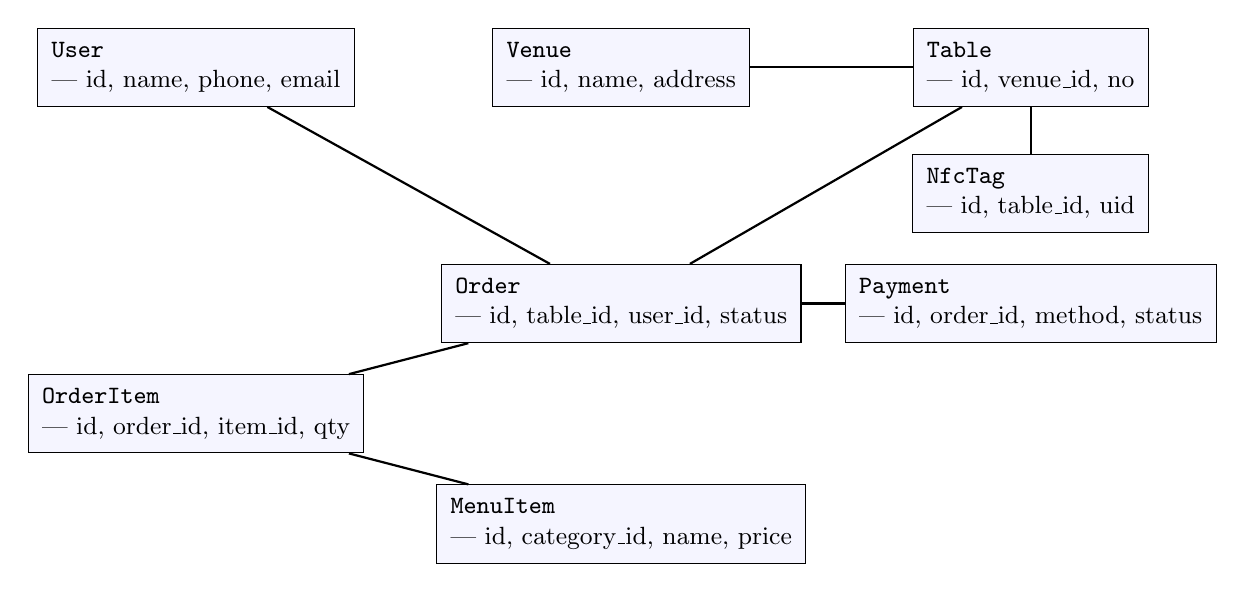
\begin{tikzpicture}
    \node[ent] (user) at (0,0) {\texttt{User}\\--- id, name, phone, email};
    \node[ent] (venue) at (5.4,0) {\texttt{Venue}\\--- id, name, address};
    \node[ent] (table) at (10.6,0) {\texttt{Table}\\--- id, venue\_id, no};
    \node[ent] (nfctag) at (10.6,-1.6) {\texttt{NfcTag}\\--- id, table\_id, uid};
    \node[ent] (order) at (5.4,-3.0) {\texttt{Order}\\--- id, table\_id, user\_id, status};
    \node[ent] (orderitem) at (0,-4.4) {\texttt{OrderItem}\\--- id, order\_id, item\_id, qty};
    \node[ent] (menuitem) at (5.4,-5.8) {\texttt{MenuItem}\\--- id, category\_id, name, price};
    \node[ent] (payment) at (10.6,-3.0) {\texttt{Payment}\\--- id, order\_id, method, status};
    \draw[thick] (user) -- (order);
    \draw[thick] (venue) -- (table);
    \draw[thick] (table) -- (nfctag);
    \draw[thick] (table) -- (order);
    \draw[thick] (order) -- (orderitem);
    \draw[thick] (orderitem) -- (menuitem);
    \draw[thick] (order) -- (payment);
  \end{tikzpicture}
  \caption{Өгөгдлийн сангийн объект-харилцааны (ER) диаграмм}
  \label{fig:ch5-er}
\end{figure}

\section{REST API-ийн тодорхойлолт}

\begin{table}[h]
  \centering
  \caption{REST API-ийн үндсэн endpoint-ууд}
  \label{tab:ch5-api}
  \small
  \begin{tabular}{@{}p{2.0cm}p{5.6cm}p{6.4cm}@{}}
    \toprule
    \textbf{HTTP} & \textbf{Endpoint} & \textbf{Тайлбар} \\ \midrule
    GET & \texttt{/api/v1/menu?venue=\{id\}} & Салбарын цэс, ангилал,
          үнийг авах \\
    POST & \texttt{/api/v1/orders} & Шинэ захиалга үүсгэх (ширеэний
           NFC стикерийн uid-ээр) \\
    GET & \texttt{/api/v1/orders/\{id\}} & Захиалгын төлөв, дэлгэрэнгүй
          мэдээлэл \\
    POST & \texttt{/api/v1/payments/intent} & Төлбөрийн санал (intent)
           үүсгэх \\
    POST & \texttt{/api/v1/payments/webhook} & Төлбөрийн үйлчилгээ
           үзүүлэгчийн callback \\
    PATCH & \texttt{/api/v1/staff/orders/\{id\}} & Ажилтан захиалгын
            төлөвийг шилжүүлэх \\
    GET & \texttt{/api/v1/admin/reports} & Орлого, захиалгын тайлан \\
    \bottomrule
  \end{tabular}
\end{table}

\section{Аюулгүй байдлын загвар}

\begin{itemize}
  \item \textbf{Бүх урсгал HTTPS:} TLS 1.2+ протокол, HSTS header
        \cite{rfc9110}.
  \item \textbf{Шошгоны кодчилол:} NFC стикерийн uid-ийг сервер дээр
        баталгаажуулж, шууд бүртгэлээс хамгаалах.
  \item \textbf{Хандалтын эрх:} RBAC (role-based access control) --
        хэрэглэгч, ажилтан, админ гэсэн 3 түвшний эрх
        \cite{owasp}.
  \item \textbf{Төлбөрийн мэдээлэл:} Картын мэдээллийг систем
        хадгалахгүй; төлбөрийн үйлчилгээ үзүүлэгчийн SDK-гаар
        шууд дамжуулна (PCI DSS-ийн шаардлага хангасан \cite{pcidss}).
  \item \textbf{Хувийн мэдээлэл:} «Хувийн нууцын тухай» хуулийн
        дагуу цуглуулсан мэдээллийг зөвхөн үйлчилгээнд шаардлагатай хэмжээнд хадгалж, хугацаа нь болоход устгана
        \cite{privacylaw}.
  \item \textbf{Аудит:} Нэвтрэлт, захиалга, төлбөрийн өөрчлөлтийг
        AuditLog хүснэгтэд хадгалж, гүйлгээний ул мөрийг бүрэн
        мөшгөх \cite{iso27001}.
\end{itemize}

\section{Хөгжүүлэлтийн төлөвлөгөө}

Төслийг 6 сарын хугацаанд 4 үе шаттайгаар хэрэгжүүлнэ
(Хүснэгт~\ref{tab:ch5-tolovlogoo}).

\begin{table}[h]
  \centering
  \caption{Хөгжүүлэлтийн үе шатууд}
  \label{tab:ch5-tolovlogoo}
  \small
  \begin{tabular}{@{}p{1.0cm}p{4.6cm}p{3.6cm}p{4.0cm}@{}}
    \toprule
    \textbf{№} & \textbf{Үе шат} & \textbf{Хугацаа} & \textbf{Гарц (deliverable)} \\
    \midrule
    1 & Шаардлага тодорхойлолт, архитектурын зураглал & 1 -- 2 сар &
    Шаардлагын баримт, диаграммууд \\
    2 & Backend болон өгөгдлийн сангийн хөгжүүлэлт & 2 -- 3 сар &
    REST API, ER бүтэц, төлбөрийн интеграци \\
    3 & PWA болон ажилтны хэсгийн хөгжүүлэлт & 3 -- 5 сар &
    Цэс, захиалга, төлбөрийн интерфэйс \\
    4 & Интеграц, тест, нэвтрүүлэг & 5 -- 6 сар &
    Бүтээгдэхүүний эхний хувилбар (MVP) \\
    \bottomrule
  \end{tabular}
\end{table}

\section{Туршилтын төлөвлөгөө}

\begin{itemize}
  \item \textbf{Нэгж туршилт:} Backend-ийн үндсэн модулиуд (захиалга
        үүсгэх, төлбөрийн intent, төлөвийн шилжилт).
  \item \textbf{Интеграцын туршилт:} NFC → цэс → захиалга → төлбөр →
        ажилтны хүлээн авалт.
  \item \textbf{Хэрэглэгчийн туршилт (UAT):} Анхдагч хэрэглэгч кофе шопт 2 -- 4
        долоо хоногийн турш бодит орчинд турших.
  \item \textbf{Ачааллын туршилт:} Оройн оргил цагт нэг салбарт
        200 -- 500 захиалга/цагийн ачааллыг тэсвэрлэх.
  \item \textbf{Аюулгүй байдлын туршилт:} HTTPS, RBAC, webhook
        баталгаажуулалтын туршилт.
\end{itemize}

% =====================================================================
%  ЗУРГАА. САНХҮҮГИЙН ТӨЛӨВЛӨГӨӨ
% =====================================================================
\chapter{САНХҮҮГИЙН ТӨЛӨВЛӨГӨӨ}

\section{Үйлдвэрлэлийн зардлын тооцоо}

Төслийн хэвийн ажиллагаанд шилжсэний дараах сар бүрийн тогтмол
зардал (Хүснэгт~\ref{tab:ch6-zardal}).

\begin{table}[h]
  \centering
  \caption{Сар бүрийн үйл ажиллагааны зардал /төгрөг/}
  \label{tab:ch6-zardal}
  \small
  \begin{tabular}{@{}p{0.8cm}p{7.6cm}r@{}}
    \toprule
    \textbf{№} & \textbf{Зардлын төрөл} & \textbf{Сарын дүн} \\
    \midrule
    1 & Cloud сервер, CDN, хадгаламж & 300{,}000 \\
    2 & Техник хангамжийн дэмжлэг, засвар үйлчилгээ & 250{,}000 \\
    3 & Ажилтны цалин (үйлчилгээний баг, 3 хүн) & 2{,}500{,}000 \\
    4 & Даатгал, НДШ & 315{,}000 \\
    5 & Маркетинг, хэрэглэгч татах зардал & 400{,}000 \\
    6 & Кофе шопын стикер солих, нэмэлт тоног төхөөрөмж & 100{,}000 \\
    7 & Бусад (офис, тээвэр, нөөц) & 235{,}000 \\
    \midrule
    & \textbf{Нийт} & \textbf{4{,}100{,}000} \\
    \bottomrule
  \end{tabular}
\end{table}

\section{Үйлдвэрлэлийн орлогын тооцоо (Борлуулалтын төлөвлөгөө)}

Орлогын гол эх үүсвэр нь кофе шопуудад зарах нэг удаагийн багц үнэ юм.
Урьдчилсан тооцоог Хүснэгт~\ref{tab:ch6-orlogo}~—т харуулав.

\begin{table}[h]
  \centering
  \caption{Борлуулалтын урьдчилсан тооцоо /төгрөг/}
  \label{tab:ch6-orlogo}
  \small
  \begin{tabular}{@{}p{0.8cm}p{4.4cm}rrr@{}}
    \toprule
    \textbf{№} & \textbf{Үзүүлэлт} & \textbf{1-р жил} & \textbf{2-р жил} &
    \textbf{3-р жил} \\ \midrule
    1 & Борлуулсан кофе шоп (Багц) & 15 & 25 & 40 \\
    2 & Багцын дундаж үнэ & 3{,}300{,}000 & 3{,}500{,}000 & 3{,}700{,}000 \\
    3 & Багцын борлуулалтын орлого & 49{,}500{,}000 & 87{,}500{,}000 & 148{,}000{,}000 \\
    4 & Нэмэлт стикер, жилийн дэмжлэгийн орлого & 3{,}000{,}000 &
        10{,}000{,}000 & 15{,}000{,}000 \\
    5 & \textbf{Нийт орлого} & \textbf{52{,}500{,}000} &
        \textbf{97{,}500{,}000} & \textbf{163{,}000{,}000} \\
    \bottomrule
  \end{tabular}
\end{table}

\section{Орлого, зардлын нэгдсэн тооцоолол}

\begin{table}[h]
  \centering
  \caption{Орлого, зардлын нэгдсэн тооцоолол /төгрөг/}
  \label{tab:ch6-negtetsen}
  \small
  \begin{tabular}{@{}p{0.6cm}p{6.4cm}rrr@{}}
    \toprule
    \textbf{№} & \textbf{Үзүүлэлт} & \textbf{1-р жил} & \textbf{2-р жил} &
    \textbf{3-р жил} \\ \midrule
    1 & Нийт орлого & 52{,}500{,}000 & 97{,}500{,}000 & 163{,}000{,}000 \\
    2 & Үйл ажиллагааны зардал (4.1\,сая x 12) & 49{,}200{,}000 &
        60{,}000{,}000 & 80{,}000{,}000 \\
    3 & Өгөгдөл хадгалах, API-ийн нэмэлт зардал & 3{,}000{,}000 &
        6{,}000{,}000 & 9{,}000{,}000 \\
    4 & ТТӨА (өмнөх) & 300{,}000 & 31{,}500{,}000 & 74{,}000{,}000 \\
    5 & Корпорацийн албан татвар (10\%) & 30{,}000 & 3{,}150{,}000 & 7{,}400{,}000 \\
    6 & \textbf{Цэвэр ашиг} & \textbf{270{,}000} &
        \textbf{28{,}350{,}000} & \textbf{66{,}600{,}000} \\
    \bottomrule
  \end{tabular}
\end{table}

\noindent 1-р жилд хөгжүүлэлтийн зардлыг хөрөнгө оруулалтад тусгаж
ажиллагааны зардлыг орлогоор бүрэн хамруулах түвшинд ажиллахаар
төлөвлөв. 2-р жилээс тогтвортой ашигтай ажиллана.

\section{Хөрөнгө оруулалтын тооцоо}

Төслийг хэрэгжүүлэхэд шаардагдах нийт хөрөнгө оруулалтыг
Хүснэгт~\ref{tab:ch6-hurungoo}~—т тусгав.

\begin{table}[h]
  \centering
  \caption{Хөрөнгө оруулалтын нийт зардал /төгрөг/}
  \label{tab:ch6-hurungoo}
  \small
  \begin{tabular}{@{}p{0.8cm}p{8.2cm}r@{}}
    \toprule
    \textbf{№} & \textbf{Хөрөнгө оруулалтын төрөл} & \textbf{Дүн} \\
    \midrule
    1 & NFC стикер, үйлчилгээний төхөөрөмж (300 ширээ) & 2{,}000{,}000 \\
    2 & Хөгжүүлэлтийн тоног төхөөрөмж (компьютер, тест утас) & 5{,}000{,}000 \\
    3 & Програм хангамжийн хөгжүүлэлт (6 сарын багийн зардал) & 34{,}185{,}360 \\
    4 & Cloud сервер, домайн, SSL (1 жил) & 2{,}400{,}000 \\
    5 & Төлбөрийн интеграци, лиценз, нотолгоо & 1{,}500{,}000 \\
    6 & Маркетинг, нэвтрүүлгийн зардал & 3{,}000{,}000 \\
    7 & Ажлын байрны зардал (6 сар) & 2{,}400{,}000 \\
    8 & Хөгжлийн нөөц (10\%) & 5{,}048{,}536 \\
    \midrule
    & \textbf{Нийт дүн} & \textbf{55{,}533{,}896} \\
    \bottomrule
  \end{tabular}
\end{table}

\noindent Тэмдэглэл: Хөгжүүлэлтийн зардлыг санхүүгийн тооцоонд
бүрэн хэмжээгээр оруулсан бөгөөд дараагийн үе шатанд бүтээгдэхүүний
хөгжүүлэлт орлогоороо санхүүжигдэнэ.

\section{Хөрөнгө оруулалтын үр ашиг}

\subsection{Хөрөнгө оруулалтын өгөөж (ROI)}

\begin{equation}
  ROI = \frac{\text{3 жилийн нийт цэвэр ашиг}}{\text{Нийт хөрөнгө оруулалт}}
      = \frac{95{,}220{,}000}{55{,}533{,}896} \approx 1.71 \; (171\%)
\end{equation}

\noindent Энэ нь нэгж хөрөнгө оруулалт тутамд 3 жилийн хугацаанд
1.71 төгрөгийн цэвэр ашиг олохоор байна гэсэн үг.

\subsection{Хөрөнгө оруулалтыг нөхөх хугацаа}

2-р жилээс эхлэн сар бүр 2{,}362{,}500\textcurrency{} (28{,}350{,}000 / 12)
цэвэр ашиг олохоор тооцсон үзүүлэлтээр, нийт хөрөнгө оруулалтын
1-р жилийн төгсгөлд үлдсэн хэсгийг нөхөхөд:

\begin{equation}
  \text{Нөхөх хугацаа} \approx 12 + \frac{55{,}263{,}896}{2{,}362{,}500}
  \approx 35 \text{ сар}
\end{equation}

\noindent Өөрөөр хэлбэл, төсөл эхэлснээс хойш ойролцоогоор 35 сарын
дотор хөрөнгө оруулалтаа бүрэн нөхөж, ажиллагааны зардлаа орлогоороо
бүрэн хамруулах түвшинд хүрнэ (борлуулалтын эрчмээс хамаарна).

\noindent Хөгжүүлэлтийн зардлыг (34{,}185{,}360\textcurrency{})
хуримтлагдсан цэвэр ашигаар нөхөхийг тооцвол: 1-р жилийн 270{,}000\textcurrency{}
ба 2-р жилийн сар бүрийн 2{,}362{,}500\textcurrency{} ашигаар
хөгжүүлэлтийн зардлыг ойролцоогоор 26 сарын дотор (3-р жилийн
дунд үе) бүрэн нөхөнө. Ингэснээр 3-р жилийн цэвэр ашиг
(66{,}600{,}000\textcurrency{}) бүхэлдээ хөрөнгө оруулалтын өгөөж болно.

\section{Зээлийн эргэн төлөлтийн тооцоо}

Хөрөнгө оруулалтын 50\% (27{,}766{,}948\textcurrency{}) нь 3 жилийн
хугацаатай, жилд 12\%-ийн хүүтэй зээлээр хангагдана
(Хүснэгт~\ref{tab:ch6-zeel}).

\begin{table}[h]
  \centering
  \caption{Төслийн зээлийн төлөлтийн график /төгрөг/}
  \label{tab:ch6-zeel}
  \small
  \begin{tabular}{@{}p{1.4cm}p{2.2cm}rrrr@{}}
    \toprule
    \textbf{Он} & \textbf{Төлөх сар} & \textbf{Үндсэн төлбөр} &
    \textbf{Зээлийн хүү} & \textbf{Нийт төлбөр} & \textbf{Зээлийн
    үлдэгдэл} \\ \midrule
    1 & 12-р сар & 9{,}255{,}649 & 3{,}332{,}034 & 12{,}587{,}683 &
    18{,}511{,}299 \\
    2 & 24-р сар & 9{,}255{,}649 & 2{,}221{,}356 & 11{,}477{,}005 &
    9{,}255{,}650 \\
    3 & 36-р сар & 9{,}255{,}650 & 1{,}110{,}678 & 10{,}366{,}328 & 0 \\
    \midrule
    & \textbf{Нийт} & \textbf{27{,}766{,}948} & \textbf{6{,}664{,}068} &
    \textbf{34{,}431{,}016} & \\
    \bottomrule
  \end{tabular}
\end{table}

% =====================================================================
%  ДОЛОО. ТӨСЛИЙН ДҮГНЭЛТ
% =====================================================================
\chapter{ТӨСЛИЙН ДҮГНЭЛТ}

\section{Төсөл хэрэгжих урьдчилсан нөхцөл, хүлээх үүрэг}

Төсөл амжилттай хэрэгжихийн тулд дараах урьдчилсан нөхцөлүүд
шийдвэрлэгдсэн байх шаардлагатай:

\begin{itemize}
  \item Хөрөнгө оруулалтын санхүүжилт (өөрийн + зээл) цагтаа
        хангагдсан байх.
  \item Төлбөрийн үйлчилгээ үзүүлэгчидтэй (QPay, SocialPay, карт
        процессинг) гэрээ байгуулсан байх.
  \item Анхдагч хэрэглэгч кофе шопуудтай хамтын ажиллагааны
        гэрээ байгуулсан байх.
  \item NFC стикер, тестийн тоног төхөөрөмж худалдаж авсан байх.
  \item Багийн бүрэн бүрэлдэхүүн ажилдаа ороод, хөгжүүлэлтийн орчин
        (cloud, repository, CI/CD \cite{githubactions}) бэлэн болсон байх.
\end{itemize}

\noindent\textbf{Хүлээх үүрэг:} Төсөл хэрэгжүүлэгч баг нь дээрх
нөхцөлүүдийг хангах, төслийн хугацаа, төсвийн дагуу гүйцэтгэх,
бүтээгдэхүүний чанарын стандартыг баримтлах үүрэг хүлээнэ. Салбар
эзэмшигч талууд нь NFC стикерийг ширээнд зөв байрлуулах, ажилтнуудаа
сургах, санал хүсэлтээ бодит цагт илгээх үүрэгтэй.

\section{Төслийн хэрэгжилтээс гарах үр дүн}

\begin{itemize}
  \item NFC стикер + PWA-д суурилсан, кассын дараалалгүй захиалга,
        төлбөрийн бүрэн системийг 6 сарын дотор бүтээн байгуулах.
  \item Эхний жилд 10 -- 20 кофе шопт бүтээгдэхүүнээ борлуулж,
        системийн тогтвортой ажиллагааг бодит орчинд батлах.
  \item Захиалгын 30 -- 40\% нь NFC урсгалаар өгөгдөх түвшинд
        хэрэглэгчдийг шилжүүлэх.
  \item Системийн таталтын ажиллагаа 99.5\%, дундаж хариу 1 секундын
        доор байх үзүүлэлтэд хүрэх.
\end{itemize}

\section{Төслийг хэрэгжүүлснээр гарах үр дүн}

\begin{itemize}
  \item \textbf{Үйлчлүүлэгчид:} Хүлээх хугацаа 40 -- 50\% багассан,
        нэг алхамаар захиалга өгөх, төлөх орчин бүрдэнэ.
  \item \textbf{Салбарууд:} Кассын ачаалал 20 -- 30\% хэмнэгдэж,
        цэс удирдах, тайлан тооцоо автоматжирана.
  \item \textbf{Төсөл хэрэгжүүлэгчид:} 3 жилийн дотор 171\%-ийн ROI,
        ойролцоогоор 35 сарын дотор хөрөнгө оруулалтаа бүрэн нөхөх
        санхүүгийн үр дүнд хүрнэ.
  \item \textbf{Салбар, эдийн засагт:} Дотоодын технологийн бүтээгдэхүүн
        нэмэгдэж, уламжлалт үйлчилгээний салбарын цифржилт хурдасна.
\end{itemize}

\section{Төслийг хэрэгжүүлснээр гарч болох эрсдлээс хамгаалах арга зам}

\begin{table}[h]
  \centering
  \caption{Эрсдэлийн үнэлгээ, хамгаалах арга зам}
  \label{tab:ch7-ersdel}
  \small
  \begin{tabular}{@{}p{0.8cm}p{3.6cm}cp{2.4cm}p{5.2cm}@{}}
    \toprule
    \textbf{№} & \textbf{Эрсдэл} & \textbf{Магадлал} & \textbf{Нөлөөлөл} &
    \textbf{Хамгаалах арга зам} \\ \midrule
    1 & Төлбөрийн үйлчилгээ үзүүлэгчийн интеграци хугацаандаа
        хоцрох & Дунд & Өндөр & Эхний үе шатнаас төлбөрийн
        документтай ажиллаж, sandbox орчинд эрт турших \\
    2 & Хэрэглэгчид NFC-ийг ойлгохгүй, QR руу буцах & Дунд & Дунд &
        Салбарын зааварчилгаа, NFC стикерийн дээр ойлгомжтой заавар
        байрлуулах, ажилтны сургалт \\
    3 & Томоохон компани ижил шийдлийг хурдан гаргах & Бага & Өндөр &
        Анхдагч хэрэглэгч кофе шопуудтай урт хугацааны хамтын
        ажиллагаа, салбарын өгөгдлийн давуу талыг бэхжүүлэх \\
    4 & Серверийн доголдол, үйлчилгээ тасалдах & Бага & Өндөр &
        Cloud-ийн өндөр хүчин чадал, автомат нөөцлөлт, мониторинг,
        offline кэш режим \\
    5 & Хувийн мэдээлэл алдагдах & Бага & Өндөр & Картын мэдээлэл
        хадгалахгүй байх, RBAC, аудитын лог, TLS, тогтмол аюулгүй
        байдлын туршилт \\
    6 & Хөгжүүлэгчийн бүрэлдэхүүн солигдох & Дунд & Дунд &
        Технологийн баримт бичгийг тогтмол хөтлөх, кодын хяналт,
        мэдлэг солилцох дотоод сургалт \\
    \bottomrule
  \end{tabular}
\end{table}

\noindent Эрсдэл бүрийг сар бүрийн төслийн хуралдаанд хянаж,
магадлал болон нөлөөллийн үнэлгээгээ шинэчилж, шаардлагатай
тохиолдолд хамгаалах арга хэмжээгээ нэмж төлөвлөнө.


% =====================================================================
%  НОМ ЗҮЙ
% =====================================================================
\addcontentsline{toc}{chapter}{Ном зүй}
\begin{thebibliography}{19}

\bibitem{iso14443}
ISO/IEC 14443, \textit{Identification cards --- Contactless integrated circuit
cards --- Proximity cards}, International Organization for Standardization,
Geneva.

\bibitem{nfcforum}
NFC Forum, \textit{NFC Forum Technical Specifications},
\url{https://nfc-forum.org}.

\bibitem{nxpntag}
NXP Semiconductors, \textit{NTAG 213/215/216 --- NFC Forum Type 2 Tag compliant
IC with 144/504/888 bytes user memory}, Product data sheet,
\url{https://www.nxp.com}.

\bibitem{coskun2012}
V. Coskun, K. Ok, B. Ozdenizci, \textit{Professional NFC Application
Development for Android}, Wiley, 2012.

\bibitem{androidnfc}
Google, \textit{NFC basics}, Android Developers documentation,
\url{https://developer.android.com/guide/topics/connectivity/nfc}.

\bibitem{corenfc}
Apple Inc., \textit{Core NFC}, Apple Developer documentation,
\url{https://developer.apple.com/documentation/corenfc}.

\bibitem{react}
Meta Open Source, \textit{React --- The library for web and native user
interfaces}, \url{https://react.dev}.

\bibitem{nestjs}
NestJS, \textit{A progressive Node.js framework for building efficient,
reliable and scalable server-side applications}, \url{https://docs.nestjs.com}.

\bibitem{postgres}
The PostgreSQL Global Development Group, \textit{PostgreSQL Documentation},
\url{https://www.postgresql.org/docs/}.

\bibitem{docker}
Docker Inc., \textit{Docker Documentation}, \url{https://docs.docker.com}.

\bibitem{playwright}
Microsoft, \textit{Playwright --- Reliable end-to-end testing for modern web
apps}, \url{https://playwright.dev}.

\bibitem{sommerville2016}
I. Sommerville, \textit{Software Engineering}, 10th ed., Pearson, 2016.

\bibitem{fielding2000}
R. T. Fielding, \textit{Architectural Styles and the Design of
Network-based Software Architectures}, PhD dissertation, University of
California, Irvine, 2000.

\bibitem{rfc9110}
R. Fielding, M. Nottingham, J. Reschke (Eds.), \textit{HTTP Semantics
(RFC 9110)}, Internet Engineering Task Force, 2022,
\url{https://www.rfc-editor.org/rfc/rfc9110}.

\bibitem{owasp}
OWASP Foundation, \textit{OWASP Top 10:2021 --- The Ten Most Critical
Web Application Security Risks}, \url{https://owasp.org/Top10}.

\bibitem{pcidss}
PCI Security Standards Council, \textit{PCI DSS --- Payment Card
Industry Data Security Standard}, v4.0,
\url{https://www.pcisecuritystandards.org}.

\bibitem{iso27001}
ISO/IEC 27001, \textit{Information security, cybersecurity and privacy
protection --- Information security management systems --- Requirements},
International Organization for Standardization, Geneva.

\bibitem{githubactions}
GitHub Inc., \textit{GitHub Actions Documentation},
\url{https://docs.github.com/actions}.

\bibitem{privacylaw}
Монгол Улсын Их Хурал, \textit{Хувийн нууцын тухай хууль},
Улаанбаатар хот.

\end{thebibliography}

\end{document}
